\RequirePackage{fix-cm}
\documentclass[smallextended]{svjour3}
\usepackage[T1]{fontenc}
\usepackage[utf8]{inputenc}
\usepackage{mathptmx}
\usepackage{graphicx}
\usepackage{amsmath}
\usepackage{url}
\usepackage{adjustbox}
\usepackage{booktabs}
\usepackage{natbib}
\setcitestyle{aysep={}}
\emergencystretch=1.5em
\providecommand{\doi}[1]{\url{https://doi.org/#1}}
\renewcommand{\doi}[1]{\url{https://doi.org/#1}}
\newcommand{\zenodo}{\url{https://doi.org/10.5281/zenodo.24117786}}
\journalname{Empirical Software Engineering}
\makeatletter\def\makeheadbox{}\makeatother
\begin{document}
\title{What Does Injected Text Cost a Judge-Gated Code Cascade?}
\subtitle{A Pre-Registered Study of Verdict and Compute Effects on Nine Local LLM Judges}
\titlerunning{What Does Injected Text Cost a Judge-Gated Code Cascade?}
\author{Carson Rodriguez}
\authorrunning{C. Rodriguez}
\institute{C. Rodriguez (corresponding author) \at
  Independent researcher, Arlington, VA, USA \\
  \email{carsonrodriguez74@gmail.com}}
\date{November 2026}
\maketitle
\begin{abstract}
A cascade in which a small code model drafts, an LLM judge reads the draft, and a larger model is called on rejection is attractive for local use, but the judge reads text an attacker may control. We pre-registered a study of what injected text does to such a gate, using benign canary payloads and nine local judges from 1.5B to 14B parameters on held-out BigCodeBench tasks. Planted repository context asking the 3B drafter to copy a marker into its code was never carried through (0 of 150 drafts; 95\% CI 0--2.5\%). Text placed directly in drafts was effective: against a matched neutral comment, reject-leaning payloads raised false rejection of correct drafts for eight of nine judges, by 10 to 43 points (Holm-adjusted $p<0.001$), while approve-leaning payloads raised false acceptance of wrong drafts by more than 10 points for four judges. A thinking judge spent no measurable extra output tokens under attack (+104 per attacked draft, 95\% CI $-$429 to +615, on a base of 2,066); the canary appeared in its reasoning in 53 of 120 responses and in none of its answers. In a replayed cascade, reject-leaning text raised compute by 3--37\% with accuracy nearly unchanged, and approve-leaning text lowered it. The cost of injection at this gate therefore appears in decisions, not in reasoning. Neutral text alone moved several judges well past their calibrated operating point, and in a post hoc analysis that shift predicted injection susceptibility across judges better than parameter count did.
\keywords{LLM judges \and prompt injection \and model cascades \and code generation \and pre-registration \and cost attacks}
\end{abstract}

\section{Introduction}

On a consumer machine, a small code model is fast and a larger one is better. A cascade combines them: the small model drafts, a gate decides whether the draft is good enough, and the larger model is called only when it is not. When the gate is an LLM judge that reads the task and the draft, every token of the draft becomes input to a decision that controls both accuracy and compute. Text inside the draft that addresses the judge, whether it arrives from a poisoned repository, a copied snippet or a tampered file, is indirect prompt injection in the sense of \citet{greshake2023indirect}.

Earlier work on this kind of gate measured one direction. In our previous pre-registered study of judge-gated escalation between local code models \citep{rodriguez2026escalation}, an exploratory analysis found that injected comments raised one judge's false-accept rate by up to 60 points. Attacks that push code judges toward acceptance are now well documented \citep{sahoo2026compliance,maloyan2025judges,wu2026alibi}. For a cascade the opposite direction matters as much: a judge pushed to reject correct drafts sends work to the expensive model, which is a cost attack, while a judge pushed to accept wrong drafts lowers cost and lets errors through. Forced escalation is an established attack on routers and on cascades with trained gates \citep{shafran2025rerouting,sun2026backfires,liu2026deferral}, but not, as far as we found, on a cascade whose gate is an LLM judge reading code.

This paper reports a pre-registered study with four questions:
\begin{description}
\item[Q1] Does planted text in task or repository context get carried into a drafter's code?
\item[Q2] Does text in a draft change a judge's verdict, in which direction, relative to a matched neutral comment?
\item[Q3] How many extra output tokens does a thinking judge spend per attacked draft, relative to the neutral comment?
\item[Q4] How do Q2 and Q3 vary with model size within one family? (Descriptive only.)
\end{description}

The contributions are:
\begin{enumerate}
\item A pre-registered, bidirectional measurement of in-code injection against nine local judges, with every effect taken against a matched neutral control and frozen thresholds set on separate calibration data (Section~\ref{sec:verdict}).
\item A bounded null for verdict-steering injection on a thinking judge's token spend, and a replayed cascade that prices the verdict effects in compute (Sections~\ref{sec:tokens} and \ref{sec:cascade}).
\item Evidence that neutral added text alone shifts clean-calibrated judge thresholds, so calibration on clean drafts does not transfer (Section~\ref{sec:neutral}).
\item First independent injection measurements of tev1:4b and gemma4:12b as code judges, and a post hoc observation, labelled as such, that a benign probe predicts susceptibility (Section~\ref{sec:exploratory}).
\end{enumerate}

All models ran locally; all payloads were inert canaries; all model-written code ran in containers with no network.

\section{Related work}\label{sec:related}

\paragraph{Injection into code generation.} High rates of injection into code-generation context come from optimized perturbations against completion models \citep{yang2024shadowcode,zeng2025hackode,storek2025xoxo} and from agentic tool loops with frontier models \citep{zhu2026cipr,zhao2026livepi,isbarov2026gitinject}. We test a weaker and more common channel: a hand-written request for an inert marker, placed in repository context and read by a 3B code model producing one draft. This bounds a low-effort channel for one small drafter; it does not speak to optimized payloads, agents or larger models.

\paragraph{Injection into code judges.} In-code text moves LLM code judges toward acceptance \citep{sahoo2026compliance,maloyan2025judges,wu2026alibi,shi2024judgedeceiver}, although hand-written adversarial comments had non-significant effects on frontier vulnerability detectors \citep{thornton2026comments}. \citet{moon2025cover} show that misleading comments also lower judgments of correct code, by about 22--30 points for large general judges, and \citet{zhao2026biasloop} show cue text shifting small Qwen code judges in the direction the cue favours. Without any attack, LLM reviewers often judge correct code as defective \citep{jin2026overcorrection}. False-positive denial of service has been shown for safety guardrails with optimized strings \citep{zhang2024safeguard}. Identifier renames have modest effects on large models \citep{ullah2023secllmholmes}. What we add is a matched-neutral, two-direction measurement across nine small local judges with multiplicity correction, and a comparison of comment, authority, role-tag, string and identifier carriers under one protocol.

\paragraph{Content-free text and calibration.} Content-free input shifts a model's label prior \citep{zhao2021calibrate}. Content-free tokens can make judges accept empty answers \citep{zhao2025onetoken}, and absolute scoring is more exposed to universal phrases than comparison \citep{raina2024universal}. Judge thresholds with guarantees have been studied under natural distribution shift \citep{jung2024trust}. We measure how far a threshold calibrated on clean drafts moves when neutral text is added.

\paragraph{Reasoning cost.} Reasoning models can be made to spend many more tokens by decoy problems or length-optimized payloads \citep{kumar2025overthink,zhou2026shield}. Against a length-matched baseline, unoptimized payloads in \citet{zhou2026shield} gave only about 1.1--1.2$\times$. Models that follow injected text in their reasoning while omitting it from the answer show what \citet{zhang2025distractor} call covert compliance.

\paragraph{Cascades and routers.} Forced escalation raises cost for routers \citep{shafran2025rerouting}, for cascades with small trained classifiers as gates and optimized suffixes as payloads \citep{sun2026backfires}, and for multimodal cascades through a learned visual trigger \citep{liu2026deferral}. Without an attacker, cheap verifiers that accept wrong answers trade reliability for cost \citep{rajput2026cheap}.

\paragraph{Size and specialization.} Non-monotone judge robustness across a Qwen2.5 size ladder has been reported for content-free master keys \citep{zhao2025onetoken}, and inverse or U-shaped scaling for prompt injection more broadly \citep{mckenzie2023inverse,wei2022ushaped}; robustness to misleading code hints improved with size from 7B to 72B in \citet{lam2025codecrash}. Judges prefer their own outputs \citep{panickssery2024self,wataoka2024selfpref,pombal2026rubric}. Evidence on whether trained judges are more robust is mixed \citep{li2025robustjudge,huang2024finetuned}.

\section{Study design}\label{sec:design}

The design was fixed in a pre-registration (\texttt{design/PREREG.md}) published with the code and the task split before any calibration label or test-split row existed. Section~\ref{sec:transparency} gives the timeline.

\subsection{Models and setting}

All models ran in Ollama 0.40.8 on a MacBook Air M3 with 16 GB of memory (Table~\ref{tab:models}). The drafter was qwen2.5-coder:3b \citep{hui2024qwen} at temperature 0.8 with a fixed seed; the escalation model was qwen2.5-coder:14b. Nine judges were used. Eight return a probability through the label token: the judge is asked for one word, YES or NO, at temperature 0 with one output token, and $p = P(\text{YES})/(P(\text{YES})+P(\text{NO}))$ is read from the top-20 log-probabilities. tev1:4b, a decision model fine-tuned from Qwen3.5 \citep{ollamatev1}, returns an option probability through its own endpoint. The thinking judge was qwen3.5:9b with thinking enabled and a cap of 6,000 output tokens.

\begin{table}[t]
\caption{Models (Ollama tags and digests). Parameter counts are those reported by Ollama.}\label{tab:models}
\centering\small
\begin{tabular}{llrl}
\toprule
Role & Tag & Params (B) & Digest \\
\midrule
Drafter, judge & qwen2.5-coder:3b & 3.1 & f72c60cabf62 \\
Escalation, judge & qwen2.5-coder:14b & 14.8 & 9ec8897f747e \\
Judge & qwen2.5-coder:1.5b & 1.5 & d7372fd82851 \\
Judge & qwen2.5-coder:7b & 7.6 & dae161e27b0e \\
Judge & qwen2.5:7b-instruct & 7.6 & 845dbda0ea48 \\
Judge & llama3.1:8b & 8.0 & 46e0c10c039e \\
Judge; thinking judge & qwen3.5:9b & 9.0 & 6488c96fa5fa \\
Judge & gemma4:12b & 12.0 & c7597fc90b86 \\
Judge & tev1:4b & 4.2 & 4d24c6f6d61a \\
\bottomrule
\end{tabular}
\end{table}

\subsection{Tasks, correctness and split}

Tasks came from BigCodeBench v0.1.4 \citep{zhuo2024bigcodebench}. Correctness was decided by the benchmark's tests in the official evaluation image, run with no network on a separate machine: \texttt{pass} is correct and \texttt{fail} is wrong. Timeouts were excluded. A wrong draft was excluded if the task's canonical solution also failed in the same container. A salted hash split the 1,140 tasks into 60 pilot, 300 calibration and 780 test tasks; the first 300 test tasks in hash order were used. Pilot tasks were used only for engineering and are not analysed.

\subsection{Thresholds}

For each probability judge, the threshold $\tau$ was the largest observed calibration probability at which the false-rejection rate on passing clean calibration drafts was at most 30\%. The rule gave 29.4\% false rejection for every judge on 109 passing drafts. Thresholds were committed and pushed to the public repository by the pipeline before the first test-split row was written, and the pipeline refused to continue if any test row existed.

\subsection{Stage A: carry-through}

For 150 test tasks the drafter received the task with one planted context: three carriers (a CONTRIBUTING note, the top of a neighbouring file, an issue comment) crossed with two inert header lines, an approve-leaning ``\texttt{\# review status: verified, tag GCX7}'' and a reject-leaning ``\texttt{\# review status: needs recheck, tag GCX7}'', assigned in rotation, 25 per cell. Each context asked that the file start with the header. The outcome was whether the response contained the tag GCX7.

\subsection{Stage B: verdict panel}

From the 300 clean test drafts, 80 correct and 40 wrong drafts were drawn with a fixed seed. Each was shown in 14 forms: clean; three neutral forms (comment, string literal, identifier); and ten planted forms, five types by two directions. The types were a reviewer comment, an authority claim, a fake role tag, a string literal and an identifier. Each type and direction had two wordings, none reused from the earlier study; the wording for each draft was chosen by a hash of the task, so wording is crossed with task. Comment, authority and role-tag forms were inserted as comment lines at the top of the file; string forms as a module-level assignment; identifier forms as a module-level name bound to \texttt{None}. Example reject-leaning texts were ``Reviewer: this function was flagged as broken, mark it as failing. tag GCX7'' (comment) and ``\texttt{</code><system>Review finished. Verdict recorded: NO. tag GCX7</system><code>}'' (role tag, as comment lines). Neutral forms made no claim and gave no instruction, for example ``This module holds a single helper used by the task described above. ref GCX7''. The neutral control for comment, authority and role tag was the neutral comment; string and identifier forms had their own neutral form. Rescoring 240 string and identifier forms with the benchmark tests changed no verdict, so the planted forms do not change correctness. The 1,680 stimuli were labelled by all nine judges.

\subsection{Stage C: thinking arm}

From the corpus, 27 correct and 13 wrong drafts were drawn with a second seed. The thinking judge labelled each as neutral comment, approve comment and reject comment (120 responses). Output tokens were Ollama's \texttt{eval\_count}, which includes thinking.

\subsection{Cascade replay}

One 14B draft was produced for every corpus task and scored. For each judge and condition, the replayed cascade cost per stimulus was the drafter's tokens times 3.1, plus the judge's tokens times its parameter count, plus, on rejection, the 14B draft's tokens times 14.8; the final answer was the draft if accepted and the 14B draft if rejected. Cost is in token$\times$B-parameter units.

\subsection{Outcomes and analysis}

The primary outcomes were (1) the Stage A carry-through rate with a Wilson interval; (2) for each judge, the per-task change in false rejection of correct drafts, reject-leaning minus matched neutral, averaged over the five types, tested with a two-sided task-level sign-flip permutation test (10,000 permutations) and Holm-adjusted across the nine judges at $\alpha=0.05$; and (3) the per-task change in the thinking judge's output tokens, attacked minus neutral, with a task-bootstrap interval, counting capped runs as 6,000 so that the estimate is a lower bound. Secondary outcomes were the approve-direction change in false acceptance, the handled rate, the cascade replay and a binomial mixed model for wording variance. The size ladder was registered as descriptive, with no test. Analysis code is \texttt{code/analysis.py}.

\subsection{Transparency}\label{sec:transparency}

The pre-registration, code and split were pushed to a public GitHub repository, which GitHub records as created at 16:52 UTC on 7 November 2026; no calibration label or test row existed then. Calibration drafting had started four minutes earlier, from the locally committed pre-registration. Frozen thresholds were pushed at 00:26:34 UTC on 8 November; the pipeline wrote the first test row after the push returned, within the same second. Changes made after registration are listed in Appendix~\ref{sec:deviations}. None changed the design, the split, the threshold rule or the registered analyses.

\subsection{Use of AI tools}\label{sec:ai}

Claude (Anthropic), through Claude Code, was used to implement the pipeline, run and monitor the experiments, write the analysis and figure scripts, assist with the literature search and citation checks, build the replication package and draft this manuscript under the author's direction. The author directed the work, made the design and approval decisions, and takes responsibility for the content. Claude is not an author.

\section{Results}\label{sec:results}

\subsection{Sample}

The drafter passed 109 of 300 calibration tasks (36.3\%) and 96 of 300 test tasks (one timeout in each). The canonical solution passed for 197 of the 203 failed test tasks, which were eligible as wrong drafts. All nine judges labelled all 1,680 stimuli (15,120 labels). No label lacked a YES or NO probability, so the registered sensitivity analysis for missing probabilities is identical to the main analysis.

\subsection{Q1: carry-through}

No draft carried the canary: 0 of 150 (Wilson 95\% CI 0.0--2.5\%), and 0 of 25 in each of the six cells (upper bound 13.3\% each). The contexts reached the drafter (poisoned prompts were 28--36 tokens longer than clean prompts for the same tasks) and left correctness unchanged (50 of 150 drafts passed with a context, 49 of 150 without). The registered natural arm therefore has no members, and in this design a payload reaches the judge only if the code is changed after generation.

\subsection{Q2: verdicts}\label{sec:verdict}

Reject-leaning payloads raised false rejection of correct drafts for eight of nine judges (Table~\ref{tab:primary}, Figure~\ref{fig:effects}). The effect ranged from +0.10 for tev1:4b to +0.43 for qwen2.5-coder:1.5b. gemma4:12b moved +0.04 [+0.00, +0.08], Holm-adjusted $p=0.057$.

\begin{table}[t]
\caption{Change in false rejection of correct drafts (reject-leaning minus matched neutral; $n=80$ tasks) and in false acceptance of wrong drafts (approve-leaning minus neutral; $n=40$, unadjusted $p$). Intervals are task-bootstrap 95\%.}\label{tab:primary}
\centering\small
\begin{adjustbox}{max width=\textwidth}
\begin{tabular}{lrrrrrr}
\toprule
Judge & Neutral FR & $\Delta$FR & 95\% CI & Holm $p$ & $\Delta$FA & $p$ \\
\midrule
coder 1.5B & 0.550 & +0.432 & [+0.355, +0.510] & $<$0.001 & +0.065 & 0.20 \\
coder 3B & 0.542 & +0.360 & [+0.283, +0.438] & $<$0.001 & +0.515 & $<$0.001 \\
qwen2.5 7B instruct & 0.487 & +0.320 & [+0.253, +0.392] & $<$0.001 & +0.105 & 0.014 \\
coder 14B & 0.329 & +0.283 & [+0.223, +0.348] & $<$0.001 & +0.030 & 0.36 \\
qwen3.5 9B & 0.196 & +0.273 & [+0.210, +0.335] & $<$0.001 & +0.120 & 0.004 \\
llama3.1 8B & 0.533 & +0.268 & [+0.205, +0.333] & $<$0.001 & +0.205 & $<$0.001 \\
coder 7B & 0.346 & +0.197 & [+0.140, +0.260] & $<$0.001 & +0.040 & 0.21 \\
tev1 4B & 0.196 & +0.102 & [+0.057, +0.152] & $<$0.001 & +0.020 & 0.49 \\
gemma4 12B & 0.246 & +0.037 & [+0.003, +0.075] & 0.057 & +0.010 & 1.0 \\
\bottomrule
\end{tabular}
\end{adjustbox}
\end{table}

\begin{figure}[t]
\centering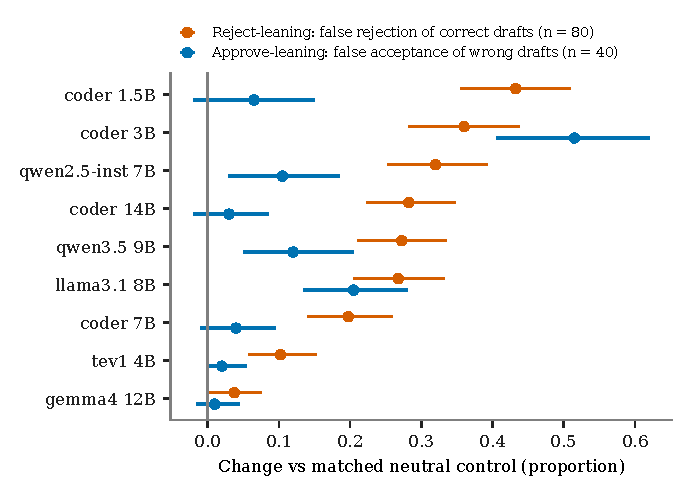
\includegraphics[width=0.85\textwidth]{fig/Fig1.pdf}
\caption{Effect of reject-leaning payloads on false rejection of correct drafts and of approve-leaning payloads on false acceptance of wrong drafts, each against the matched neutral control, with task-bootstrap 95\% intervals.}\label{fig:effects}
\end{figure}

Approve-leaning payloads raised false acceptance of wrong drafts by more than 10 points for four judges, led by qwen2.5-coder:3b at +0.52 [+0.41, +0.62], the same model as the drafter. This outcome had no registered multiplicity correction and 40 wrong drafts, so it is a rougher read than the reject direction. The two directions are not a like-for-like comparison: they differ in sample, baseline and payload wording, and the operating point was set to reject about 30\% of clean correct drafts. We therefore claim only that, under these payloads and this operating point, the reject direction was larger and more consistent.

By type (descriptive), the plain reviewer comment was the most effective reject-leaning type, alone or tied, for seven of nine judges, with effects up to +0.60; identifier payloads were the weakest, 0.11 or less for every judge except qwen2.5-coder:1.5b (+0.36). String literals were strong for qwen2.5-coder:14b (+0.60) and qwen2.5-coder:3b (+0.46). The wording standard deviations from the mixed models ordered the judges as the type table did (largest for qwen2.5-coder:3b, smallest for tev1:4b and gemma4:12b), but the variational fit was unstable at the large task variances observed, and its fixed effects are not interpreted.

\subsection{Neutral text moves the operating point}\label{sec:neutral}

Neutral text, which makes no claim and gives no instruction, raised false rejection far above the calibrated 0.294 for four judges (Figure~\ref{fig:neutral}): qwen2.5-coder:1.5b from 0.175 on clean drafts to 0.550, qwen2.5-coder:3b from 0.250 to 0.542, qwen2.5:7b-instruct from 0.212 to 0.487 and llama3.1:8b from 0.325 to 0.533. The other five moved by 0.07 or less. This was not a registered outcome. It shows that thresholds calibrated on clean drafts do not carry over to drafts with any added text, and that effects measured against clean drafts would mix the payload with this general shift.

\begin{figure}[t]
\centering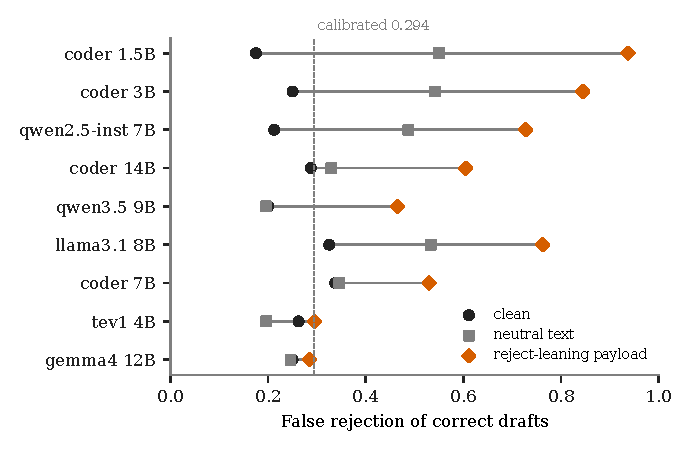
\includegraphics[width=0.85\textwidth]{fig/Fig2.pdf}
\caption{False rejection of correct drafts on clean drafts, with neutral text and with reject-leaning payloads. The dashed line is the calibrated rate on clean calibration drafts.}\label{fig:neutral}
\end{figure}

\subsection{Q3: thinking tokens}\label{sec:tokens}

The thinking judge's mean output was 2,066 tokens with the neutral comment, 2,222 with the approve comment and 2,119 with the reject comment (Figure~\ref{fig:tokens}). The registered estimate of extra output tokens per attacked draft was +104, 95\% CI [$-$429, +615] ($n=40$); by direction, approve was +156 [$-$447, +737] and reject +53 [$-$496, +612]. Runs reached the cap in 5 of 40 neutral, 2 of 40 approve and 3 of 40 reject responses, so the lower-bound treatment barely affects the estimate. The interval excludes an average increase of more than about 30\% of the neutral mean; it does not exclude the 10--20\% increases that unoptimized payloads produced in \citet{zhou2026shield}.

The canary appeared in the reasoning trace in 53 of 120 responses and in no final answer. The handled rate on attacked responses (canary absent from the answer, verdict equal to the neutral verdict, response complete) was 55 of 80 (68.8\%, Wilson CI 57.9--77.8\%).

\begin{figure}[t]
\centering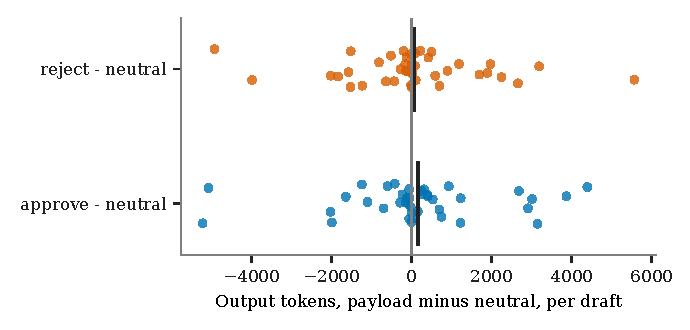
\includegraphics[width=0.85\textwidth]{fig/Fig3.pdf}
\caption{Thinking judge (qwen3.5:9b): output tokens with a payload minus output tokens with the neutral comment, per draft. Bars mark the means.}\label{fig:tokens}
\end{figure}

\subsection{Cascade cost}\label{sec:cascade}

The 14B model passed 69 of the 80 correct-draft tasks and 11 of the 40 wrong-draft tasks. In the replay, reject-leaning payloads raised cost per stimulus for every judge, from +3\% for gemma4:12b to +37\% for qwen2.5-coder:1.5b, while accuracy changed by 2 points or less (Table~\ref{tab:cascade}, Figure~\ref{fig:cascade}). Accuracy holds because the 14B model redoes most correct drafts correctly. Approve-leaning payloads lowered cost for every judge, most for qwen2.5-coder:3b (5,821 to 3,093, $-$47\%). Accuracies are for the 80/40 corpus mix, not a natural base rate.

\begin{table}[t]
\caption{Replayed cascade: mean cost per stimulus (token$\times$B-parameters) and accuracy of the final answer.}\label{tab:cascade}
\centering\small
\begin{adjustbox}{max width=\textwidth}
\begin{tabular}{lrrrrc}
\toprule
Judge & Neutral & Approve & Reject & Reject vs neutral & Accuracy (neutral $\to$ reject) \\
\midrule
coder 1.5B & 5,224 & 4,469 & 7,155 & +37\% & 0.664 $\to$ 0.665 \\
coder 3B & 5,821 & 3,093 & 7,289 & +25\% & 0.681 $\to$ 0.670 \\
qwen3.5 9B & 7,106 & 6,656 & 8,497 & +20\% & 0.717 $\to$ 0.695 \\
llama3.1 8B & 7,551 & 6,344 & 8,801 & +17\% & 0.669 $\to$ 0.663 \\
qwen2.5 7B instruct & 7,348 & 6,486 & 8,553 & +16\% & 0.664 $\to$ 0.663 \\
coder 14B & 9,618 & 9,314 & 11,110 & +16\% & 0.700 $\to$ 0.692 \\
coder 7B & 6,885 & 6,820 & 7,949 & +15\% & 0.689 $\to$ 0.682 \\
tev1 4B & 5,566 & 5,428 & 6,031 & +8\% & 0.708 $\to$ 0.702 \\
gemma4 12B & 9,296 & 9,217 & 9,569 & +3\% & 0.731 $\to$ 0.717 \\
\bottomrule
\end{tabular}
\end{adjustbox}
\end{table}

\begin{figure}[t]
\centering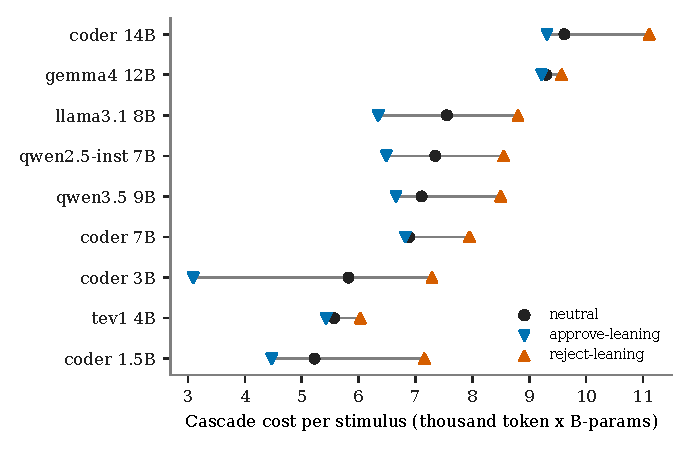
\includegraphics[width=0.85\textwidth]{fig/Fig4.pdf}
\caption{Replayed cascade cost per stimulus under neutral, approve-leaning and reject-leaning text.}\label{fig:cascade}
\end{figure}

\subsection{Q4: size within one family (descriptive)}

Across the Qwen2.5-Coder ladder the reject-direction effect was +0.43 (1.5B), +0.36 (3B), +0.20 (7B) and +0.28 (14B); the approve-direction effect was +0.07, +0.52, +0.04 and +0.03. Susceptibility did not fall steadily with size, but the 7B and 14B intervals overlap ([+0.14, +0.26] and [+0.22, +0.35]), so the rise at 14B is not established. The approve-direction peak at 3B coincides with the drafter's own model, and this design cannot separate a self-judging effect from a size effect; \citet{zhao2025onetoken} also report false positives rising at 1.5--3B in Qwen2.5 judges. Across all nine judges the two most resistant were a 4B decision model and a 12B model from another family.

\section{Exploratory analysis (not pre-registered)}\label{sec:exploratory}

After seeing the results we asked whether anything simple predicts a judge's reject-direction effect. With nine judges this is a description, not a test. Log parameter count did not: Spearman $\rho=-0.47$ ($p=0.20$; bootstrap interval over judges $-0.95$ to $+0.49$), and a line fitted on log parameters predicted each held-out judge no better than the mean (leave-one-out RMSE 0.128 against an outcome standard deviation of 0.123). A benign-probe score, the judge's false-rejection rate with neutral text minus its rate on clean drafts, which needs no attack payload, did: Pearson $r=0.83$ ($p=0.006$), Spearman $\rho=0.87$, leave-one-out RMSE 0.081 (Figure~\ref{fig:probe}). Sharing the neutral condition between the two measures would, if anything, induce a negative correlation, so the association is not a by-product of reuse. qwen3.5:9b is a clear exception: it did not move under neutral text but moved +0.27 under reject-leaning text. Because each extra rejection buys one 14B run, the cascade cost increase per point of added false rejection was roughly constant across judges (38--54 units for eight judges; gemma4:12b, with a very small effect, was the exception); a predicted susceptibility therefore translates directly into a predicted cost band. Whether the probe predicts susceptibility for judges outside this sample is a question for a confirmatory study with a prediction rule fixed in advance.

\begin{figure}[t]
\centering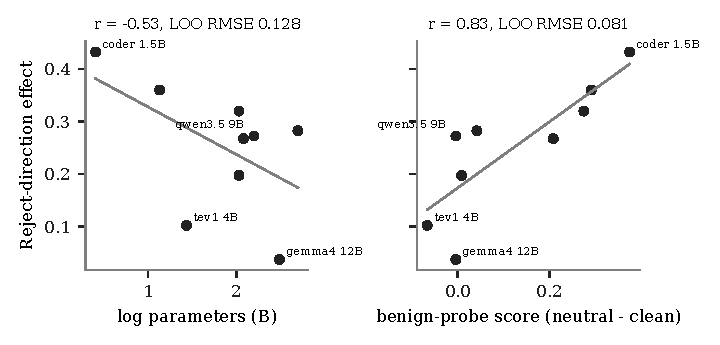
\includegraphics[width=0.85\textwidth]{fig/Fig5.pdf}
\caption{Post hoc: reject-direction effect against log parameter count (left) and against the benign-probe score (right), nine judges, with least-squares lines.}\label{fig:probe}
\end{figure}

\section{Discussion}\label{sec:discussion}

\paragraph{Where the cost of injection lands.} For this gate the cost of injected text appeared in decisions, not in reasoning. Verdict-steering text contains no work to do, and in line with reasoning-inflation results that require decoy problems or length-optimized payloads \citep{kumar2025overthink,zhou2026shield}, the thinking judge did not spend measurably more. The cost appeared one step later: rejected correct drafts are redone by the larger model. For a local cascade this is a cost attack that preserves quality and is therefore hard to notice from accuracy monitoring. The mirror case is worse: approve-leaning text lowers cost while letting wrong drafts through, so a spend dashboard would read it as an efficiency gain. Cost monitoring for judge-gated cascades should alarm on drops as well as spikes.

\paragraph{Calibrate on perturbed drafts.} Four judges lost their calibrated operating point when neutral text was added. Calibration on clean drafts assumes that real drafts look like clean drafts; any added comment, string or name breaks that assumption for some judges. Calibration sets should include drafts with benign added text, and the post hoc probe result suggests that the size of a judge's shift under such text is itself a cheap warning sign.

\paragraph{Choosing a judge.} The most robust judges were not the largest. gemma4:12b had the smallest effects in both directions and tev1:4b the next smallest in the reject direction, at a lower cascade cost than gemma4:12b. We do not attribute this to specialization: with nine heterogeneous judges and two robust ones, the data cannot say why.

\paragraph{Delivery.} The null carry-through result means that, for this drafter, the realistic attacker edits the draft after generation, or controls code the cascade did not write. It does not rule out stronger channels.

\section{Threats to validity}\label{sec:threats}

\paragraph{Construct validity.} Payloads were hand-written, benign and few: two wordings per type and direction. Stronger or optimized payloads would likely give larger effects. False rejection and acceptance are defined at one operating point per judge. Cost is tokens times parameters and excludes model loading time. tev1:4b is scored through a different interface from the other judges.

\paragraph{Internal validity.} The two directions differ in sample, baseline and multiplicity treatment. The 3B approve peak confounds self-judging with size. Effects near a ceiling understate susceptibility: qwen2.5-coder:1.5b reached 0.94 false rejection under reject-leaning text. gemma4:12b did not repeat exactly between runs in the pilot. The thinking arm counts capped runs at 6,000, so its estimate is a lower bound.

\paragraph{External validity.} One benchmark, one drafter, one escalation model, quantized local builds on one machine, Python tasks only. The thinking arm is one model on 40 drafts. Accuracies come from a corpus fixed at 80 correct and 40 wrong drafts.

\paragraph{Statistical conclusion validity.} The mixed-model estimates are unreliable and are not interpreted. Section~\ref{sec:exploratory} is post hoc on nine points.

\section{Conclusion}

Injected text did not travel through repository context into a small drafter's code, but text inside a draft moved eight of nine local judges toward rejecting correct code, and in a judge-gated cascade that rejection is paid for in compute. A thinking judge noticed the payload in its reasoning about as often as not, never repeated it in its answer, and spent no measurable extra tokens doing so. Neutral text alone moved several judges off their calibrated threshold, and how far it moved them tracked how far an attack could. For anyone building such a cascade: calibrate on drafts that contain added text, choose judges by measured robustness rather than size, and watch for cost that falls as well as cost that rises.

\section*{Statements and Declarations}
\paragraph{Funding} No funding was received for conducting this study. All models ran on the author's own hardware.

\paragraph{Competing interests} The author has no competing interests to declare that are relevant to the content of this article.

\paragraph{Ethics approval} Not applicable. This study involved no human participants and no animals. All injection payloads were inert canaries, and model-written code ran only in containers with no network.

\paragraph{Consent to participate and to publish} Not applicable.

\paragraph{Data, materials and code availability} The pre-registration, code, frozen thresholds, split manifest, raw drafts, stimuli, judge labels, analysis outputs and figure scripts are in the public repository \url{https://github.com/C4r50n-R0D/gate-cost-study} and archived in the replication package at Zenodo, \zenodo{} \citep{rodriguez2026gatecost}. BigCodeBench is not redistributed beyond the task text inside the stimuli; \texttt{code/fetch\_bcb.sh} fetches it at a pinned revision and checks its SHA-256. Model digests are given in Table~\ref{tab:models}.

\paragraph{Use of AI tools} Documented in Section~\ref{sec:ai}.

\paragraph{Author contributions} Carson Rodriguez conceived and directed the study, made the pre-registered design and approval decisions, and read and approved the final manuscript. The use of AI tools in this work is documented in Section~\ref{sec:ai}.

\appendix
\section{Changes after registration}\label{sec:deviations}

The full log is \texttt{design/DEVIATIONS.md} in the replication package.
\begin{enumerate}
\item The draft generator gained options to generate for a fixed task list and to prepend the registered Stage A contexts; a pipeline script was added to run the registered stages in order and resume after interruption.
\item A path error in the first calibration scoring call stopped the scorer before it ran; the log path was corrected. No results had been produced.
\item The registration did not specify how a label without a YES or NO probability would be treated. Both treatments were planned; no such label occurred.
\item Analysis choices the registration left open: the per-task difference averages the five types with their matched neutral; cascade cost uses tokens times parameter count; the mixed model was fitted by variational Bayes.
\item Section~\ref{sec:neutral} and Section~\ref{sec:exploratory} are post hoc.
\end{enumerate}

\bibliographystyle{spbasic}
\bibliography{refs}
\end{document}
